% This creates Beamer slides for Cohen, Jessica, Pascaline Dupas, and Simone Schaner. "Price subsidies, diagnostic tests, and targeting of malaria treatment: evidence from a randomized controlled trial." American Economic Review 105.2 (2015): 609-645.

\documentclass{beamer}

\usepackage[utf8]{inputenc} % Ensure proper encoding
\usepackage{graphicx} % For including images
\usepackage{hyperref} % For hyperlinks
\usepackage{amsmath,amsfonts,amssymb} % For mathematical symbols and equations

\setbeamertemplate{footline}[frame number] % Add page numbers

\begin{document}

\title{Price Subsidies, Diagnostic Tests, and Targeting of Malaria Treatment: Evidence from a Randomized Controlled Trial}
\author{Jessica Cohen, Pascaline Dupas, and Simone Schaner}
\date{\today}

\frame{\titlepage}

\begin{frame}{Introduction}
    \begin{itemize}
        \item Treating infectious diseases have positive spillovers and therefore they should be subsidized. 
        \item However, if product has hetrogenous returns, it is important to target subsidies where they have highest returns: Hence trade-off between targeting and accessibilty. 
        \item So essentially you want to target the group with highest returns. This is a menu-setting problem. 
    \end{itemize}
\end{frame}

\begin{frame}{This Paper}
\begin{itemize}
    \item This paper studies the menu-setting problem introduced by subsidies for the latest class of antimalarials in Kenya.
    \item This durg is very useful if the patient has malaria but people usually take drug without being tested and hence presumptive treatment is common.
    \item Over treatment can also contribute to parasite resistance rendering drug ineffective in future.
    \item Usually you would have public health system where diagnostic tools and trained medical personnel can target technologies to patients with high returns. However, if public health system is weak or inaccessible, then this is not possible.
    \item Alternative is to give subsidized drugs through retail sector. 
    \item Importantly, beneficiaries are not mimicking the high return group but rather they also don't have information about their malaria status.
\end{itemize}
\end{frame}


\begin{frame}{Experimental Design}
\begin{itemize}

    \item The experiment  conducted with over 2,700 households in Western Kenya, introduced random variation in
    access to heavily subsidized ACTs and rapid tests sold through local drug shops and monitored the impact on treatment seeking behavior and medication taking.
    


\end{itemize}
\begin{figure}

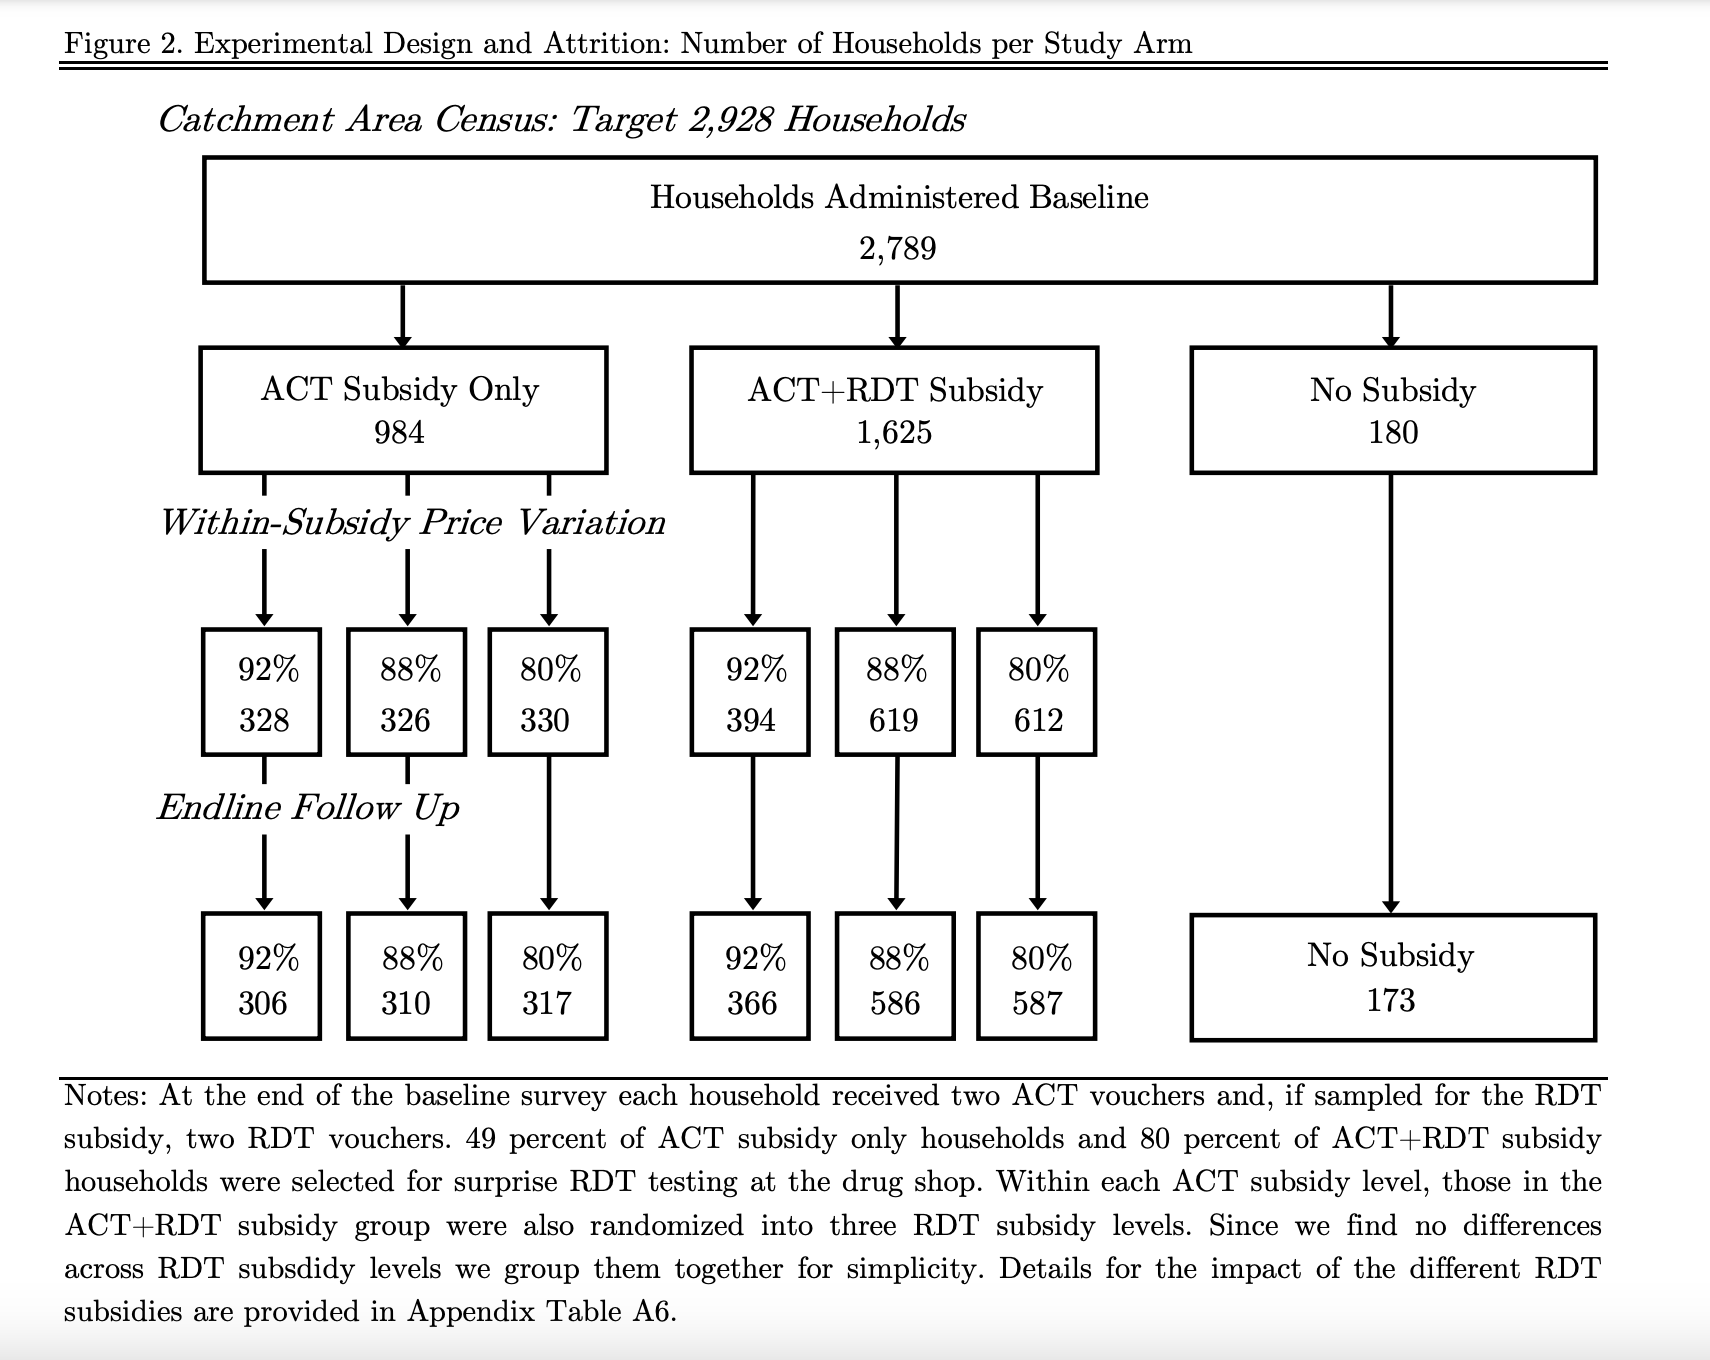
\includegraphics[width=0.5\textwidth]{F2.png}
\end{figure}
    \end{frame}

\begin{frame}[allowframebreaks]{Results}  
\begin{enumerate}
\item Many households bypass the public system
entirely and instead procure medication through retail-sector drug shops.
\item So heavy retail sector subsidy increases targeting. However, this increase is among both appropriate and inappropriate users and hence overall targeting is not great. Only 56\% of those who bought the drug had malaria.
\item Decreasing subsidy from 92\% to 80\% increases targeting without much loss to accessibility and therefore trade-off is not that severe.

    \end{enumerate}
\end{frame}

\begin{frame}{ACT demand by subsidy level}
\begin{figure}
    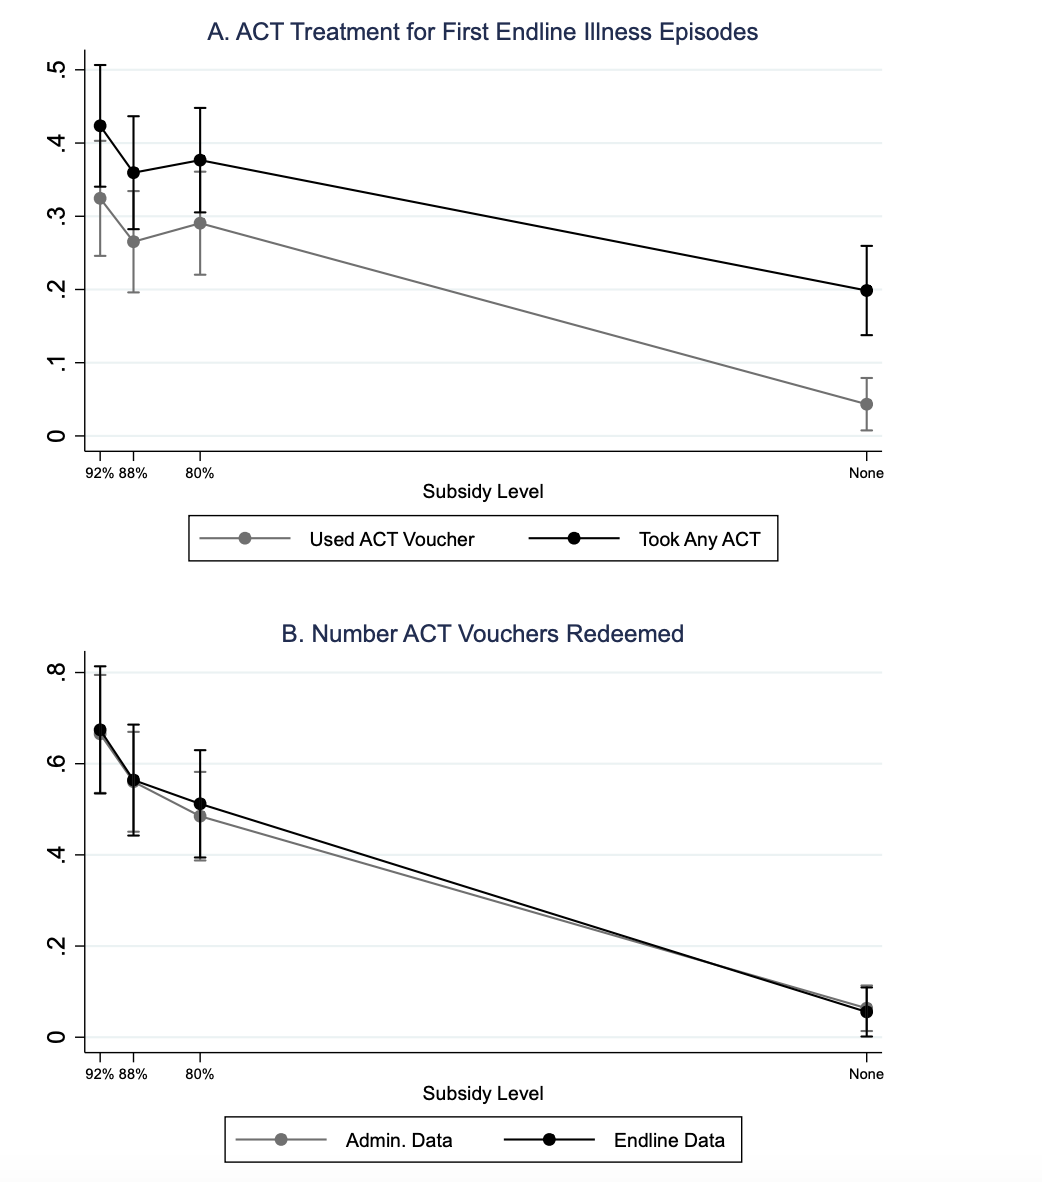
\includegraphics[width=0.8\textwidth, height=0.8\textheight]{F4.png}
\end{figure}
    \end{frame}

    \begin{frame}{Compliance by subsidy level}
        \begin{figure}
            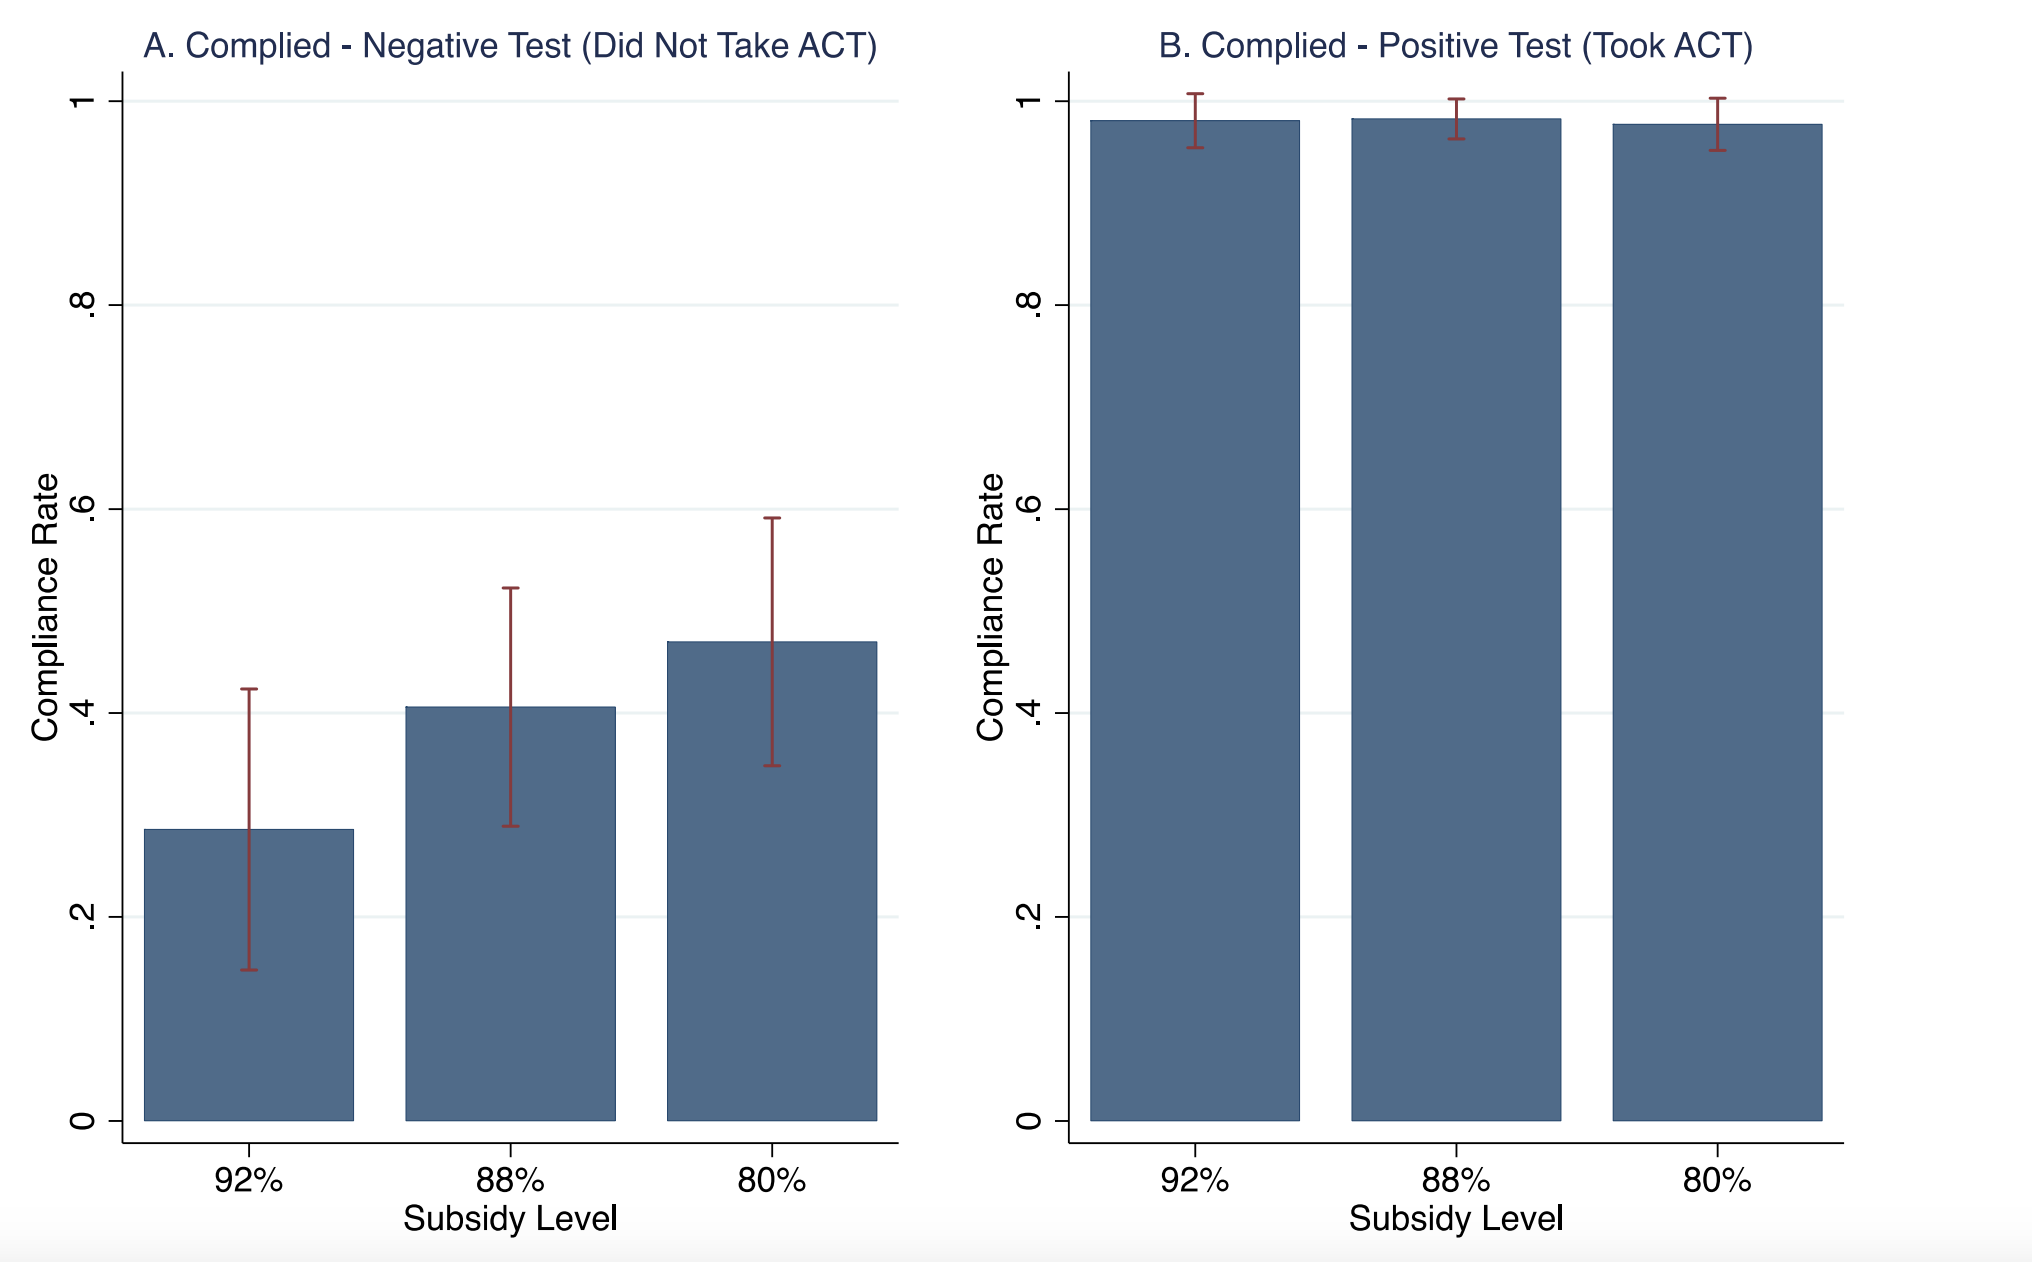
\includegraphics[width=\textwidth]{F5.png}
        \end{figure}
            \end{frame}

\begin{frame}{Impact of Subsidy on Targeting}
\begin{figure}
    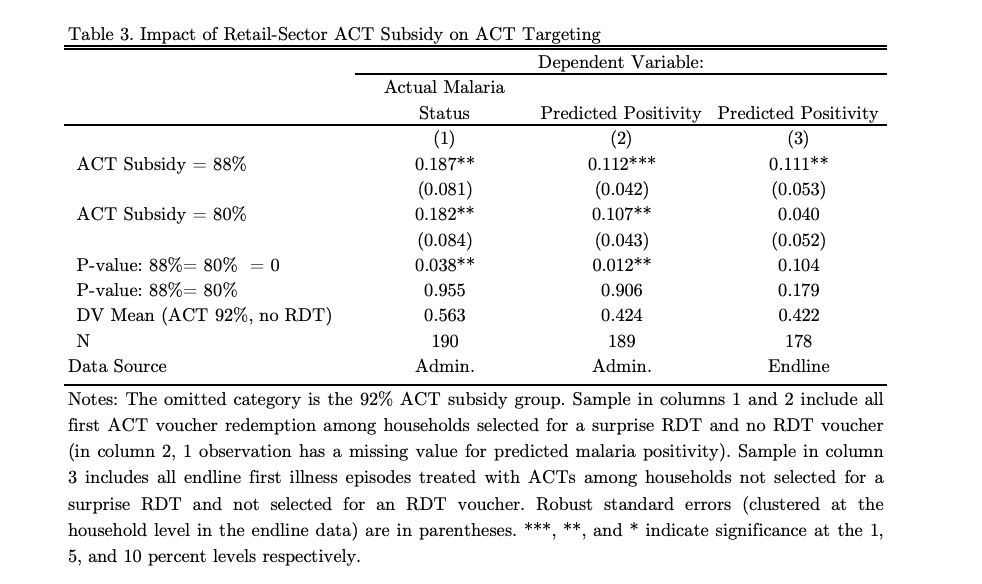
\includegraphics[width=0.8\textwidth, height=0.8\textheight]{T3.png}
\end{figure}
\end{frame}

\begin{frame}{Mechanisms: Where does targeting improve?}
\begin{figure}
    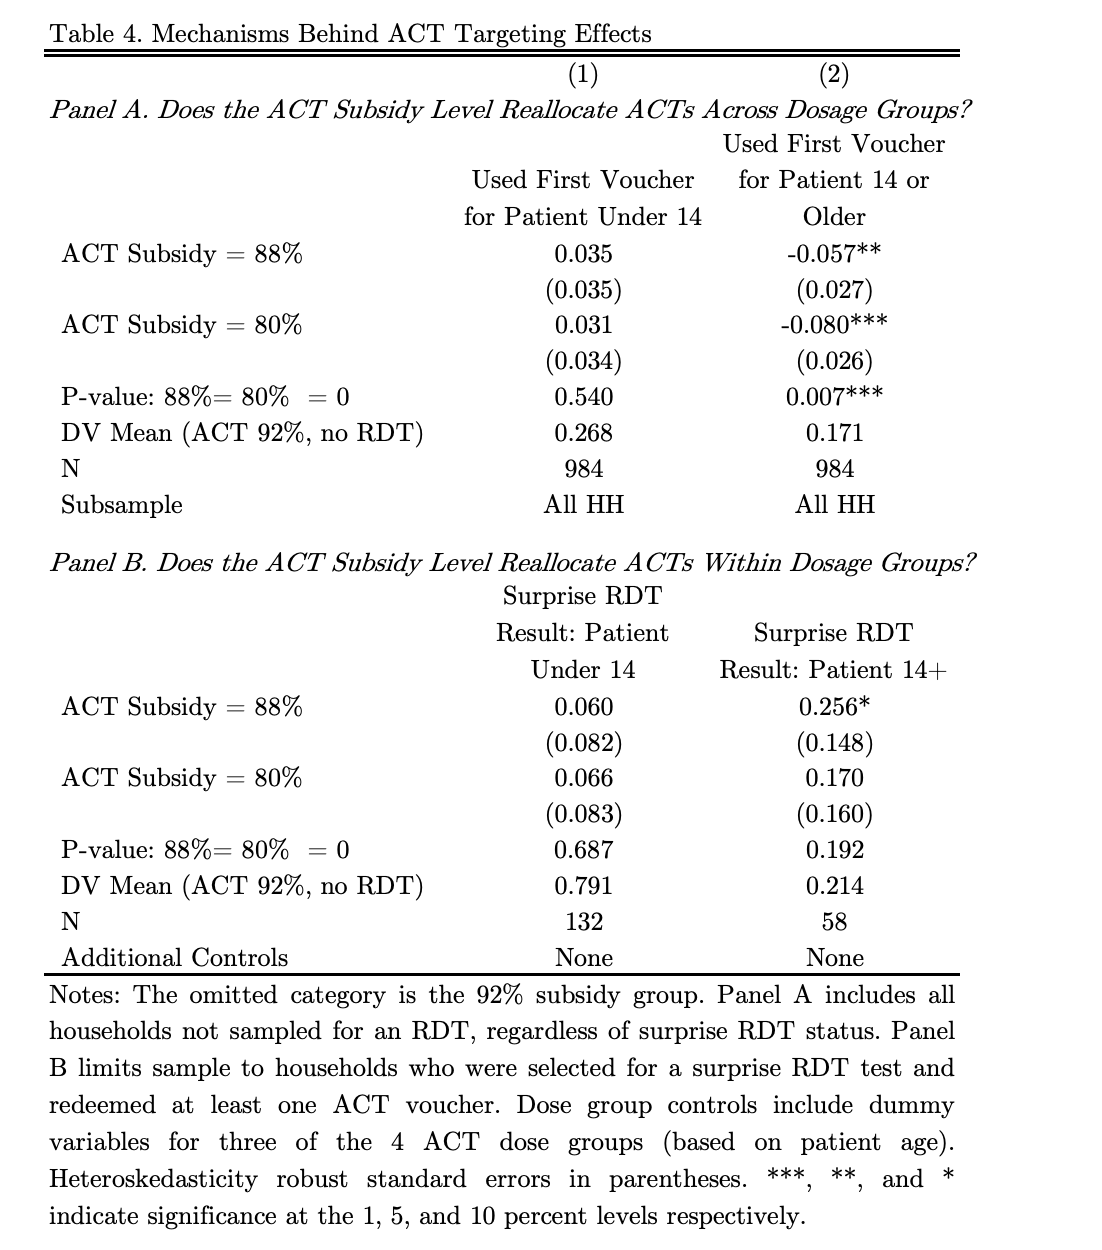
\includegraphics[width=0.8\textwidth, height=0.8\textheight]{T4.png}
\end{figure}

\end{frame}

\begin{frame}{Estimated Impacts of Various Subsidy Schemes on Under- and Over-Treatment}
    \begin{figure}
        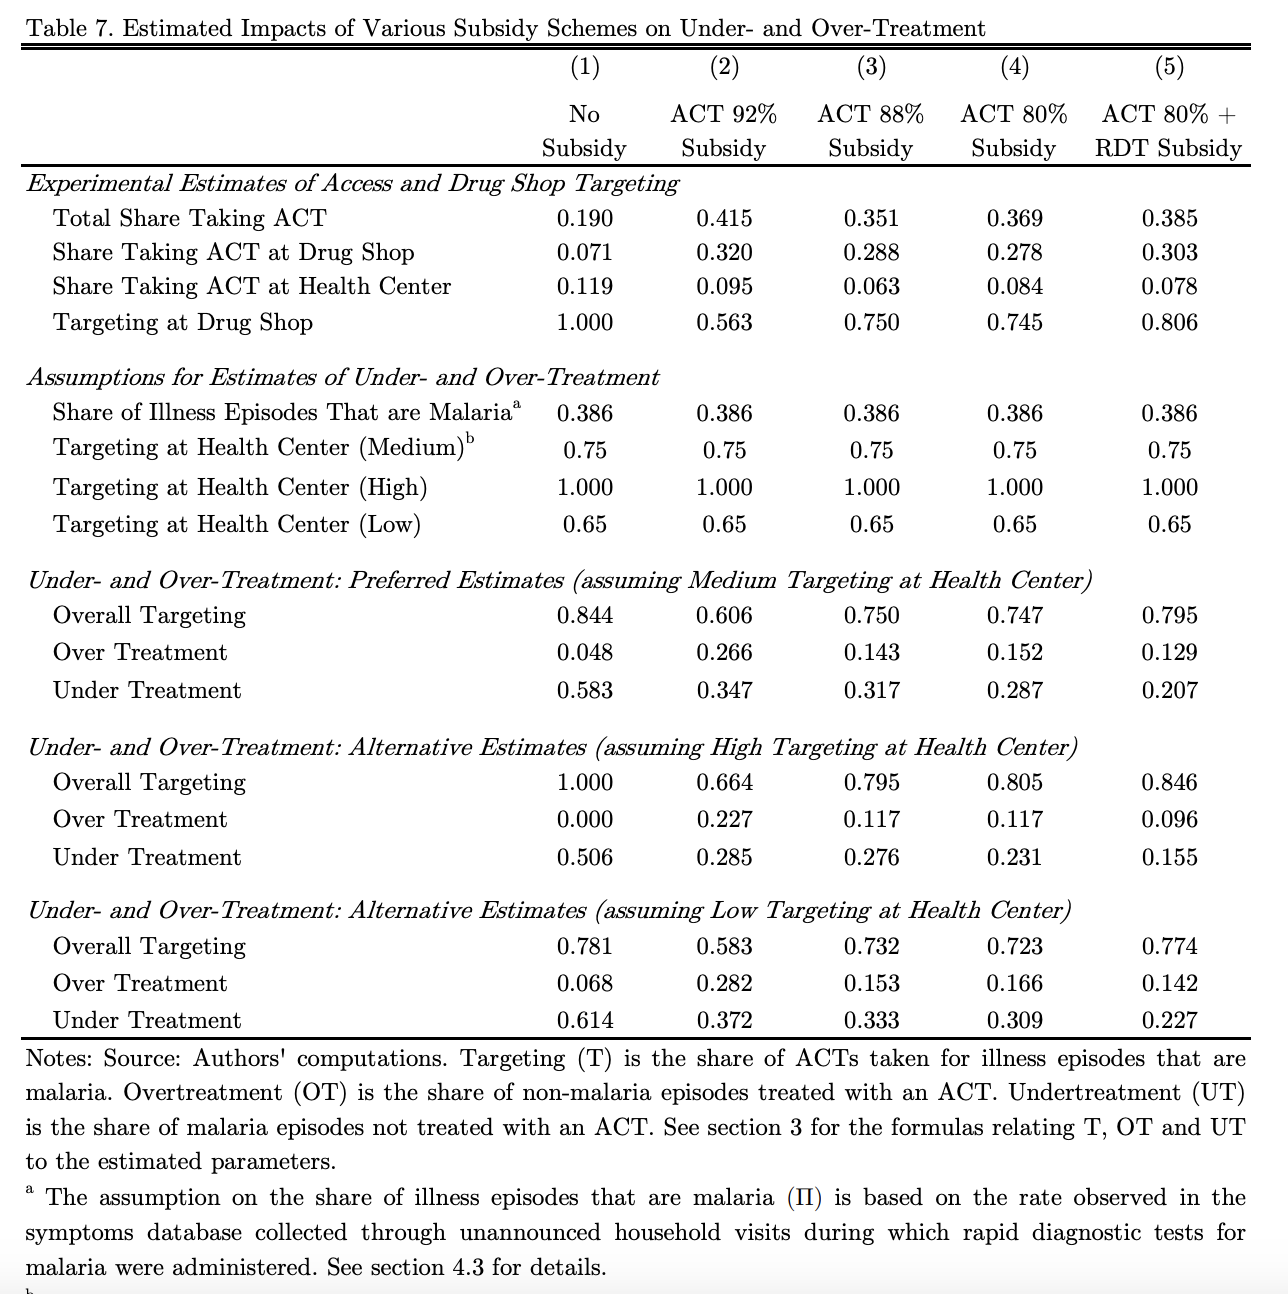
\includegraphics[width=0.8\textwidth, height=0.8\textheight]{T7.png}
    \end{figure}
\end{frame}

\end{document}